% !TEX encoding = UTF-8 Unicode
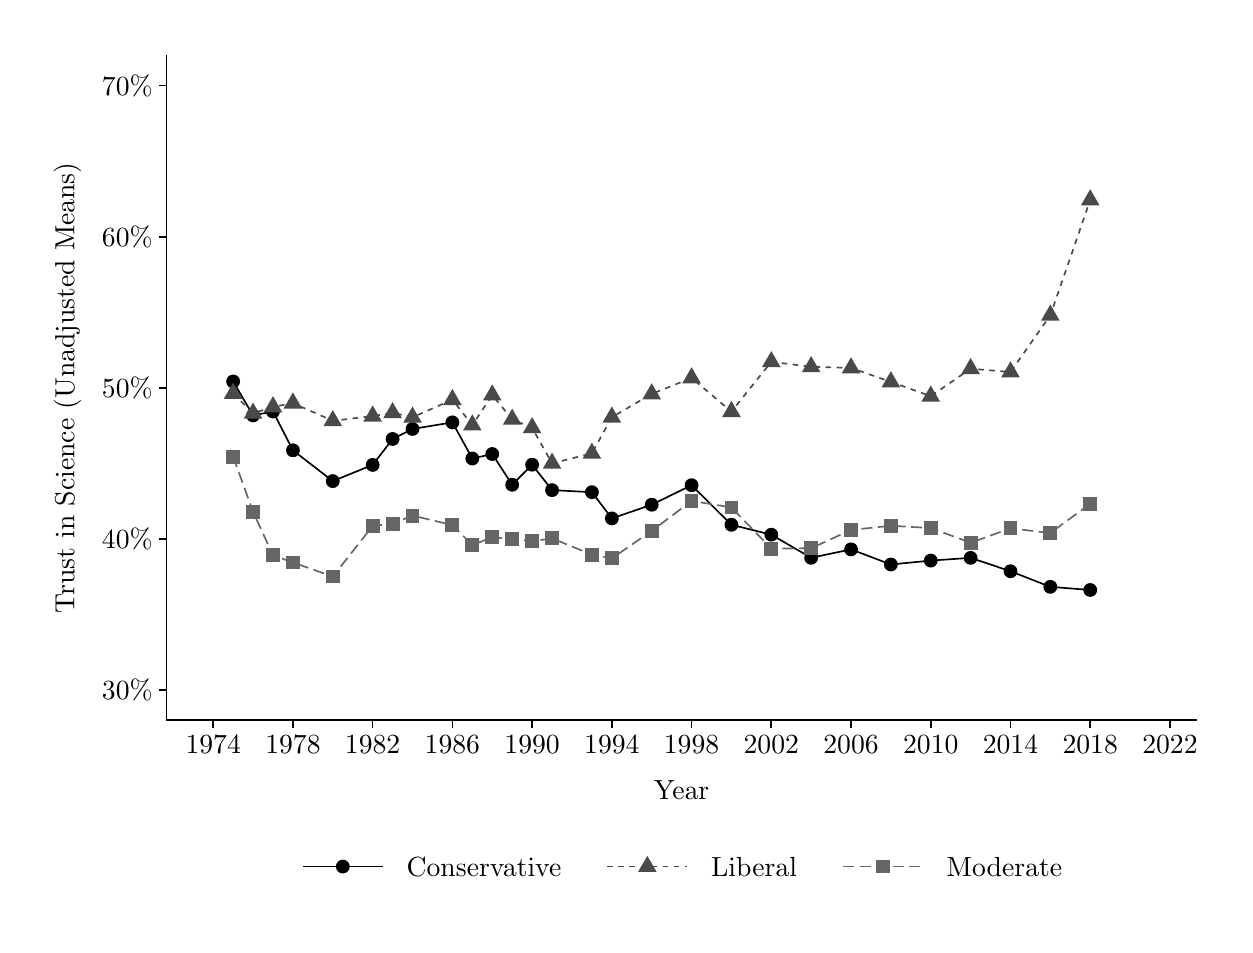
\begin{tikzpicture}[x=1pt,y=1pt]
\definecolor{fillColor}{RGB}{255,255,255}
\path[use as bounding box,fill=fillColor,fill opacity=0.00] (0,0) rectangle (432.48,324.36);
\begin{scope}
\path[clip] (  0.00,  0.00) rectangle (432.48,324.36);
\definecolor{fillColor}{RGB}{255,255,255}

\path[fill=fillColor] ( -0.00,  0.00) rectangle (432.48,324.36);
\end{scope}
\begin{scope}
\path[clip] ( 50.11, 74.07) rectangle (422.48,314.36);
\definecolor{fillColor}{RGB}{255,255,255}

\path[fill=fillColor] ( 50.11, 74.07) rectangle (422.48,314.36);
\definecolor{drawColor}{RGB}{0,0,0}

\path[draw=drawColor,line width= 0.6pt,line join=round] ( 74.24,196.52) --
	( 81.44,184.25) --
	( 88.64,185.66) --
	( 95.85,171.64) --
	(110.25,160.51) --
	(124.66,166.36) --
	(131.86,175.73) --
	(139.06,179.36) --
	(153.47,181.73) --
	(160.67,168.67) --
	(167.87,170.30) --
	(175.07,159.19) --
	(182.28,166.44) --
	(189.48,157.25) --
	(203.88,156.51) --
	(211.09,147.03) --
	(225.49,151.98) --
	(239.90,159.02) --
	(254.30,144.73) --
	(268.71,141.15) --
	(283.11,132.80) --
	(297.52,135.84) --
	(311.92,130.38) --
	(326.33,131.79) --
	(340.73,132.78) --
	(355.14,127.94) --
	(369.54,122.30) --
	(383.95,121.17);
\definecolor{drawColor}{gray}{0.29}

\path[draw=drawColor,line width= 0.6pt,dash pattern=on 2pt off 2pt ,line join=round] ( 74.24,192.20) --
	( 81.44,185.01) --
	( 88.64,187.33) --
	( 95.85,188.68) --
	(110.25,182.30) --
	(124.66,183.98) --
	(131.86,185.20) --
	(139.06,183.58) --
	(153.47,189.94) --
	(160.67,180.75) --
	(167.87,191.59) --
	(175.07,182.82) --
	(182.28,179.77) --
	(189.48,166.93) --
	(203.88,170.53) --
	(211.09,183.60) --
	(225.49,192.01) --
	(239.90,197.78) --
	(254.30,185.61) --
	(268.71,203.63) --
	(283.11,201.81) --
	(297.52,201.40) --
	(311.92,196.36) --
	(326.33,191.19) --
	(340.73,201.13) --
	(355.14,199.94) --
	(369.54,220.43) --
	(383.95,262.10);
\definecolor{drawColor}{gray}{0.40}

\path[draw=drawColor,line width= 0.6pt,dash pattern=on 4pt off 2pt ,line join=round] ( 74.24,169.35) --
	( 81.44,149.41) --
	( 88.64,133.73) --
	( 95.85,131.10) --
	(110.25,126.03) --
	(124.66,144.28) --
	(131.86,145.11) --
	(139.06,148.04) --
	(153.47,144.64) --
	(160.67,137.36) --
	(167.87,140.27) --
	(175.07,139.51) --
	(182.28,138.79) --
	(189.48,139.82) --
	(203.88,133.92) --
	(211.09,132.58) --
	(225.49,142.51) --
	(239.90,153.34) --
	(254.30,151.01) --
	(268.71,136.12) --
	(283.11,136.25) --
	(297.52,142.87) --
	(311.92,144.37) --
	(326.33,143.55) --
	(340.73,138.25) --
	(355.14,143.44) --
	(369.54,141.76) --
	(383.95,152.31);
\definecolor{fillColor}{RGB}{0,0,0}

\path[fill=fillColor] ( 74.24,196.52) circle (  2.50);
\definecolor{fillColor}{gray}{0.29}

\path[fill=fillColor] ( 74.24,196.09) --
	( 77.60,190.26) --
	( 70.87,190.26) --
	cycle;
\definecolor{fillColor}{gray}{0.40}

\path[fill=fillColor] ( 71.74,166.85) --
	( 76.74,166.85) --
	( 76.74,171.85) --
	( 71.74,171.85) --
	cycle;
\definecolor{fillColor}{RGB}{0,0,0}

\path[fill=fillColor] ( 81.44,184.25) circle (  2.50);
\definecolor{fillColor}{gray}{0.29}

\path[fill=fillColor] ( 81.44,188.89) --
	( 84.80,183.07) --
	( 78.08,183.07) --
	cycle;
\definecolor{fillColor}{gray}{0.40}

\path[fill=fillColor] ( 78.94,146.91) --
	( 83.94,146.91) --
	( 83.94,151.90) --
	( 78.94,151.90) --
	cycle;
\definecolor{fillColor}{RGB}{0,0,0}

\path[fill=fillColor] ( 88.64,185.66) circle (  2.50);
\definecolor{fillColor}{gray}{0.29}

\path[fill=fillColor] ( 88.64,191.21) --
	( 92.01,185.38) --
	( 85.28,185.38) --
	cycle;
\definecolor{fillColor}{gray}{0.40}

\path[fill=fillColor] ( 86.15,131.24) --
	( 91.14,131.24) --
	( 91.14,136.23) --
	( 86.15,136.23) --
	cycle;
\definecolor{fillColor}{RGB}{0,0,0}

\path[fill=fillColor] ( 95.85,171.64) circle (  2.50);
\definecolor{fillColor}{gray}{0.29}

\path[fill=fillColor] ( 95.85,192.56) --
	( 99.21,186.74) --
	( 92.48,186.74) --
	cycle;
\definecolor{fillColor}{gray}{0.40}

\path[fill=fillColor] ( 93.35,128.60) --
	( 98.34,128.60) --
	( 98.34,133.60) --
	( 93.35,133.60) --
	cycle;
\definecolor{fillColor}{RGB}{0,0,0}

\path[fill=fillColor] (110.25,160.51) circle (  2.50);
\definecolor{fillColor}{gray}{0.29}

\path[fill=fillColor] (110.25,186.18) --
	(113.62,180.36) --
	(106.89,180.36) --
	cycle;
\definecolor{fillColor}{gray}{0.40}

\path[fill=fillColor] (107.75,123.53) --
	(112.75,123.53) --
	(112.75,128.53) --
	(107.75,128.53) --
	cycle;
\definecolor{fillColor}{RGB}{0,0,0}

\path[fill=fillColor] (124.66,166.36) circle (  2.50);
\definecolor{fillColor}{gray}{0.29}

\path[fill=fillColor] (124.66,187.87) --
	(128.02,182.04) --
	(121.29,182.04) --
	cycle;
\definecolor{fillColor}{gray}{0.40}

\path[fill=fillColor] (122.16,141.78) --
	(127.15,141.78) --
	(127.15,146.78) --
	(122.16,146.78) --
	cycle;
\definecolor{fillColor}{RGB}{0,0,0}

\path[fill=fillColor] (131.86,175.73) circle (  2.50);
\definecolor{fillColor}{gray}{0.29}

\path[fill=fillColor] (131.86,189.08) --
	(135.22,183.25) --
	(128.50,183.25) --
	cycle;
\definecolor{fillColor}{gray}{0.40}

\path[fill=fillColor] (129.36,142.61) --
	(134.36,142.61) --
	(134.36,147.61) --
	(129.36,147.61) --
	cycle;
\definecolor{fillColor}{RGB}{0,0,0}

\path[fill=fillColor] (139.06,179.36) circle (  2.50);
\definecolor{fillColor}{gray}{0.29}

\path[fill=fillColor] (139.06,187.47) --
	(142.43,181.64) --
	(135.70,181.64) --
	cycle;
\definecolor{fillColor}{gray}{0.40}

\path[fill=fillColor] (136.56,145.54) --
	(141.56,145.54) --
	(141.56,150.54) --
	(136.56,150.54) --
	cycle;
\definecolor{fillColor}{RGB}{0,0,0}

\path[fill=fillColor] (153.47,181.73) circle (  2.50);
\definecolor{fillColor}{gray}{0.29}

\path[fill=fillColor] (153.47,193.82) --
	(156.83,187.99) --
	(150.10,187.99) --
	cycle;
\definecolor{fillColor}{gray}{0.40}

\path[fill=fillColor] (150.97,142.15) --
	(155.96,142.15) --
	(155.96,147.14) --
	(150.97,147.14) --
	cycle;
\definecolor{fillColor}{RGB}{0,0,0}

\path[fill=fillColor] (160.67,168.67) circle (  2.50);
\definecolor{fillColor}{gray}{0.29}

\path[fill=fillColor] (160.67,184.63) --
	(164.03,178.80) --
	(157.31,178.80) --
	cycle;
\definecolor{fillColor}{gray}{0.40}

\path[fill=fillColor] (158.17,134.86) --
	(163.17,134.86) --
	(163.17,139.86) --
	(158.17,139.86) --
	cycle;
\definecolor{fillColor}{RGB}{0,0,0}

\path[fill=fillColor] (167.87,170.30) circle (  2.50);
\definecolor{fillColor}{gray}{0.29}

\path[fill=fillColor] (167.87,195.47) --
	(171.24,189.64) --
	(164.51,189.64) --
	cycle;
\definecolor{fillColor}{gray}{0.40}

\path[fill=fillColor] (165.37,137.77) --
	(170.37,137.77) --
	(170.37,142.77) --
	(165.37,142.77) --
	cycle;
\definecolor{fillColor}{RGB}{0,0,0}

\path[fill=fillColor] (175.07,159.19) circle (  2.50);
\definecolor{fillColor}{gray}{0.29}

\path[fill=fillColor] (175.07,186.70) --
	(178.44,180.88) --
	(171.71,180.88) --
	cycle;
\definecolor{fillColor}{gray}{0.40}

\path[fill=fillColor] (172.58,137.01) --
	(177.57,137.01) --
	(177.57,142.00) --
	(172.58,142.00) --
	cycle;
\definecolor{fillColor}{RGB}{0,0,0}

\path[fill=fillColor] (182.28,166.44) circle (  2.50);
\definecolor{fillColor}{gray}{0.29}

\path[fill=fillColor] (182.28,183.65) --
	(185.64,177.83) --
	(178.91,177.83) --
	cycle;
\definecolor{fillColor}{gray}{0.40}

\path[fill=fillColor] (179.78,136.30) --
	(184.77,136.30) --
	(184.77,141.29) --
	(179.78,141.29) --
	cycle;
\definecolor{fillColor}{RGB}{0,0,0}

\path[fill=fillColor] (189.48,157.25) circle (  2.50);
\definecolor{fillColor}{gray}{0.29}

\path[fill=fillColor] (189.48,170.82) --
	(192.84,164.99) --
	(186.12,164.99) --
	cycle;
\definecolor{fillColor}{gray}{0.40}

\path[fill=fillColor] (186.98,137.33) --
	(191.98,137.33) --
	(191.98,142.32) --
	(186.98,142.32) --
	cycle;
\definecolor{fillColor}{RGB}{0,0,0}

\path[fill=fillColor] (203.88,156.51) circle (  2.50);
\definecolor{fillColor}{gray}{0.29}

\path[fill=fillColor] (203.88,174.42) --
	(207.25,168.59) --
	(200.52,168.59) --
	cycle;
\definecolor{fillColor}{gray}{0.40}

\path[fill=fillColor] (201.39,131.43) --
	(206.38,131.43) --
	(206.38,136.42) --
	(201.39,136.42) --
	cycle;
\definecolor{fillColor}{RGB}{0,0,0}

\path[fill=fillColor] (211.09,147.03) circle (  2.50);
\definecolor{fillColor}{gray}{0.29}

\path[fill=fillColor] (211.09,187.49) --
	(214.45,181.66) --
	(207.72,181.66) --
	cycle;
\definecolor{fillColor}{gray}{0.40}

\path[fill=fillColor] (208.59,130.08) --
	(213.58,130.08) --
	(213.58,135.08) --
	(208.59,135.08) --
	cycle;
\definecolor{fillColor}{RGB}{0,0,0}

\path[fill=fillColor] (225.49,151.98) circle (  2.50);
\definecolor{fillColor}{gray}{0.29}

\path[fill=fillColor] (225.49,195.89) --
	(228.86,190.06) --
	(222.13,190.06) --
	cycle;
\definecolor{fillColor}{gray}{0.40}

\path[fill=fillColor] (222.99,140.01) --
	(227.99,140.01) --
	(227.99,145.00) --
	(222.99,145.00) --
	cycle;
\definecolor{fillColor}{RGB}{0,0,0}

\path[fill=fillColor] (239.90,159.02) circle (  2.50);
\definecolor{fillColor}{gray}{0.29}

\path[fill=fillColor] (239.90,201.66) --
	(243.26,195.83) --
	(236.53,195.83) --
	cycle;
\definecolor{fillColor}{gray}{0.40}

\path[fill=fillColor] (237.40,150.85) --
	(242.39,150.85) --
	(242.39,155.84) --
	(237.40,155.84) --
	cycle;
\definecolor{fillColor}{RGB}{0,0,0}

\path[fill=fillColor] (254.30,144.73) circle (  2.50);
\definecolor{fillColor}{gray}{0.29}

\path[fill=fillColor] (254.30,189.50) --
	(257.67,183.67) --
	(250.94,183.67) --
	cycle;
\definecolor{fillColor}{gray}{0.40}

\path[fill=fillColor] (251.80,148.51) --
	(256.80,148.51) --
	(256.80,153.50) --
	(251.80,153.50) --
	cycle;
\definecolor{fillColor}{RGB}{0,0,0}

\path[fill=fillColor] (268.71,141.15) circle (  2.50);
\definecolor{fillColor}{gray}{0.29}

\path[fill=fillColor] (268.71,207.51) --
	(272.07,201.69) --
	(265.34,201.69) --
	cycle;
\definecolor{fillColor}{gray}{0.40}

\path[fill=fillColor] (266.21,133.62) --
	(271.21,133.62) --
	(271.21,138.62) --
	(266.21,138.62) --
	cycle;
\definecolor{fillColor}{RGB}{0,0,0}

\path[fill=fillColor] (283.11,132.80) circle (  2.50);
\definecolor{fillColor}{gray}{0.29}

\path[fill=fillColor] (283.11,205.70) --
	(286.48,199.87) --
	(279.75,199.87) --
	cycle;
\definecolor{fillColor}{gray}{0.40}

\path[fill=fillColor] (280.61,133.75) --
	(285.61,133.75) --
	(285.61,138.74) --
	(280.61,138.74) --
	cycle;
\definecolor{fillColor}{RGB}{0,0,0}

\path[fill=fillColor] (297.52,135.84) circle (  2.50);
\definecolor{fillColor}{gray}{0.29}

\path[fill=fillColor] (297.52,205.28) --
	(300.88,199.46) --
	(294.15,199.46) --
	cycle;
\definecolor{fillColor}{gray}{0.40}

\path[fill=fillColor] (295.02,140.37) --
	(300.02,140.37) --
	(300.02,145.36) --
	(295.02,145.36) --
	cycle;
\definecolor{fillColor}{RGB}{0,0,0}

\path[fill=fillColor] (311.92,130.38) circle (  2.50);
\definecolor{fillColor}{gray}{0.29}

\path[fill=fillColor] (311.92,200.24) --
	(315.29,194.41) --
	(308.56,194.41) --
	cycle;
\definecolor{fillColor}{gray}{0.40}

\path[fill=fillColor] (309.43,141.87) --
	(314.42,141.87) --
	(314.42,146.86) --
	(309.43,146.86) --
	cycle;
\definecolor{fillColor}{RGB}{0,0,0}

\path[fill=fillColor] (326.33,131.79) circle (  2.50);
\definecolor{fillColor}{gray}{0.29}

\path[fill=fillColor] (326.33,195.07) --
	(329.69,189.24) --
	(322.96,189.24) --
	cycle;
\definecolor{fillColor}{gray}{0.40}

\path[fill=fillColor] (323.83,141.05) --
	(328.83,141.05) --
	(328.83,146.05) --
	(323.83,146.05) --
	cycle;
\definecolor{fillColor}{RGB}{0,0,0}

\path[fill=fillColor] (340.73,132.78) circle (  2.50);
\definecolor{fillColor}{gray}{0.29}

\path[fill=fillColor] (340.73,205.01) --
	(344.10,199.19) --
	(337.37,199.19) --
	cycle;
\definecolor{fillColor}{gray}{0.40}

\path[fill=fillColor] (338.24,135.75) --
	(343.23,135.75) --
	(343.23,140.74) --
	(338.24,140.74) --
	cycle;
\definecolor{fillColor}{RGB}{0,0,0}

\path[fill=fillColor] (355.14,127.94) circle (  2.50);
\definecolor{fillColor}{gray}{0.29}

\path[fill=fillColor] (355.14,203.82) --
	(358.50,198.00) --
	(351.77,198.00) --
	cycle;
\definecolor{fillColor}{gray}{0.40}

\path[fill=fillColor] (352.64,140.94) --
	(357.64,140.94) --
	(357.64,145.94) --
	(352.64,145.94) --
	cycle;
\definecolor{fillColor}{RGB}{0,0,0}

\path[fill=fillColor] (369.54,122.30) circle (  2.50);
\definecolor{fillColor}{gray}{0.29}

\path[fill=fillColor] (369.54,224.32) --
	(372.91,218.49) --
	(366.18,218.49) --
	cycle;
\definecolor{fillColor}{gray}{0.40}

\path[fill=fillColor] (367.05,139.26) --
	(372.04,139.26) --
	(372.04,144.26) --
	(367.05,144.26) --
	cycle;
\definecolor{fillColor}{RGB}{0,0,0}

\path[fill=fillColor] (383.95,121.17) circle (  2.50);
\definecolor{fillColor}{gray}{0.29}

\path[fill=fillColor] (383.95,265.99) --
	(387.31,260.16) --
	(380.58,260.16) --
	cycle;
\definecolor{fillColor}{gray}{0.40}

\path[fill=fillColor] (381.45,149.81) --
	(386.45,149.81) --
	(386.45,154.80) --
	(381.45,154.80) --
	cycle;
\end{scope}
\begin{scope}
\path[clip] (  0.00,  0.00) rectangle (432.48,324.36);
\definecolor{drawColor}{RGB}{0,0,0}

\path[draw=drawColor,line width= 0.6pt,line join=round] ( 50.11, 74.07) --
	( 50.11,314.36);
\end{scope}
\begin{scope}
\path[clip] (  0.00,  0.00) rectangle (432.48,324.36);
\definecolor{drawColor}{RGB}{0,0,0}

\node[text=drawColor,anchor=base east,inner sep=0pt, outer sep=0pt, scale=  1.00] at ( 45.16, 81.55) {30{\%}};

\node[text=drawColor,anchor=base east,inner sep=0pt, outer sep=0pt, scale=  1.00] at ( 45.16,136.16) {40{\%}};

\node[text=drawColor,anchor=base east,inner sep=0pt, outer sep=0pt, scale=  1.00] at ( 45.16,190.77) {50{\%}};

\node[text=drawColor,anchor=base east,inner sep=0pt, outer sep=0pt, scale=  1.00] at ( 45.16,245.38) {60{\%}};

\node[text=drawColor,anchor=base east,inner sep=0pt, outer sep=0pt, scale=  1.00] at ( 45.16,300.00) {70{\%}};
\end{scope}
\begin{scope}
\path[clip] (  0.00,  0.00) rectangle (432.48,324.36);
\definecolor{drawColor}{RGB}{0,0,0}

\path[draw=drawColor,line width= 0.6pt,line join=round] ( 47.36, 84.99) --
	( 50.11, 84.99);

\path[draw=drawColor,line width= 0.6pt,line join=round] ( 47.36,139.60) --
	( 50.11,139.60);

\path[draw=drawColor,line width= 0.6pt,line join=round] ( 47.36,194.21) --
	( 50.11,194.21);

\path[draw=drawColor,line width= 0.6pt,line join=round] ( 47.36,248.83) --
	( 50.11,248.83);

\path[draw=drawColor,line width= 0.6pt,line join=round] ( 47.36,303.44) --
	( 50.11,303.44);
\end{scope}
\begin{scope}
\path[clip] (  0.00,  0.00) rectangle (432.48,324.36);
\definecolor{drawColor}{RGB}{0,0,0}

\path[draw=drawColor,line width= 0.6pt,line join=round] ( 50.11, 74.07) --
	(422.48, 74.07);
\end{scope}
\begin{scope}
\path[clip] (  0.00,  0.00) rectangle (432.48,324.36);
\definecolor{drawColor}{RGB}{0,0,0}

\path[draw=drawColor,line width= 0.6pt,line join=round] ( 67.04, 71.32) --
	( 67.04, 74.07);

\path[draw=drawColor,line width= 0.6pt,line join=round] ( 95.85, 71.32) --
	( 95.85, 74.07);

\path[draw=drawColor,line width= 0.6pt,line join=round] (124.66, 71.32) --
	(124.66, 74.07);

\path[draw=drawColor,line width= 0.6pt,line join=round] (153.47, 71.32) --
	(153.47, 74.07);

\path[draw=drawColor,line width= 0.6pt,line join=round] (182.28, 71.32) --
	(182.28, 74.07);

\path[draw=drawColor,line width= 0.6pt,line join=round] (211.09, 71.32) --
	(211.09, 74.07);

\path[draw=drawColor,line width= 0.6pt,line join=round] (239.90, 71.32) --
	(239.90, 74.07);

\path[draw=drawColor,line width= 0.6pt,line join=round] (268.71, 71.32) --
	(268.71, 74.07);

\path[draw=drawColor,line width= 0.6pt,line join=round] (297.52, 71.32) --
	(297.52, 74.07);

\path[draw=drawColor,line width= 0.6pt,line join=round] (326.33, 71.32) --
	(326.33, 74.07);

\path[draw=drawColor,line width= 0.6pt,line join=round] (355.14, 71.32) --
	(355.14, 74.07);

\path[draw=drawColor,line width= 0.6pt,line join=round] (383.95, 71.32) --
	(383.95, 74.07);

\path[draw=drawColor,line width= 0.6pt,line join=round] (412.76, 71.32) --
	(412.76, 74.07);
\end{scope}
\begin{scope}
\path[clip] (  0.00,  0.00) rectangle (432.48,324.36);
\definecolor{drawColor}{RGB}{0,0,0}

\node[text=drawColor,anchor=base,inner sep=0pt, outer sep=0pt, scale=  1.00] at ( 67.04, 62.23) {1974};

\node[text=drawColor,anchor=base,inner sep=0pt, outer sep=0pt, scale=  1.00] at ( 95.85, 62.23) {1978};

\node[text=drawColor,anchor=base,inner sep=0pt, outer sep=0pt, scale=  1.00] at (124.66, 62.23) {1982};

\node[text=drawColor,anchor=base,inner sep=0pt, outer sep=0pt, scale=  1.00] at (153.47, 62.23) {1986};

\node[text=drawColor,anchor=base,inner sep=0pt, outer sep=0pt, scale=  1.00] at (182.28, 62.23) {1990};

\node[text=drawColor,anchor=base,inner sep=0pt, outer sep=0pt, scale=  1.00] at (211.09, 62.23) {1994};

\node[text=drawColor,anchor=base,inner sep=0pt, outer sep=0pt, scale=  1.00] at (239.90, 62.23) {1998};

\node[text=drawColor,anchor=base,inner sep=0pt, outer sep=0pt, scale=  1.00] at (268.71, 62.23) {2002};

\node[text=drawColor,anchor=base,inner sep=0pt, outer sep=0pt, scale=  1.00] at (297.52, 62.23) {2006};

\node[text=drawColor,anchor=base,inner sep=0pt, outer sep=0pt, scale=  1.00] at (326.33, 62.23) {2010};

\node[text=drawColor,anchor=base,inner sep=0pt, outer sep=0pt, scale=  1.00] at (355.14, 62.23) {2014};

\node[text=drawColor,anchor=base,inner sep=0pt, outer sep=0pt, scale=  1.00] at (383.95, 62.23) {2018};

\node[text=drawColor,anchor=base,inner sep=0pt, outer sep=0pt, scale=  1.00] at (412.76, 62.23) {2022};
\end{scope}
\begin{scope}
\path[clip] (  0.00,  0.00) rectangle (432.48,324.36);
\definecolor{drawColor}{RGB}{0,0,0}

\node[text=drawColor,anchor=base,inner sep=0pt, outer sep=0pt, scale=  1.00] at (236.30, 45.40) {Year};
\end{scope}
\begin{scope}
\path[clip] (  0.00,  0.00) rectangle (432.48,324.36);
\definecolor{drawColor}{RGB}{0,0,0}

\node[text=drawColor,rotate= 90.00,anchor=base,inner sep=0pt, outer sep=0pt, scale=  1.00] at ( 16.89,194.21) {Trust in Science (Unadjusted Means)};
\end{scope}
\begin{scope}
\path[clip] (  0.00,  0.00) rectangle (432.48,324.36);

\path[] ( 86.80, 10.00) rectangle (385.79, 32.45);
\end{scope}
\begin{scope}
\path[clip] (  0.00,  0.00) rectangle (432.48,324.36);

\path[] ( 95.80, 14.00) rectangle (131.94, 28.45);
\end{scope}
\begin{scope}
\path[clip] (  0.00,  0.00) rectangle (432.48,324.36);
\definecolor{drawColor}{RGB}{0,0,0}

\path[draw=drawColor,line width= 0.6pt,line join=round] ( 99.42, 21.23) -- (128.33, 21.23);
\end{scope}
\begin{scope}
\path[clip] (  0.00,  0.00) rectangle (432.48,324.36);
\definecolor{fillColor}{RGB}{0,0,0}

\path[fill=fillColor] (113.87, 21.23) circle (  2.50);
\end{scope}
\begin{scope}
\path[clip] (  0.00,  0.00) rectangle (432.48,324.36);

\path[] (205.84, 14.00) rectangle (241.98, 28.45);
\end{scope}
\begin{scope}
\path[clip] (  0.00,  0.00) rectangle (432.48,324.36);
\definecolor{drawColor}{gray}{0.29}

\path[draw=drawColor,line width= 0.6pt,dash pattern=on 2pt off 2pt ,line join=round] (209.46, 21.23) -- (238.36, 21.23);
\end{scope}
\begin{scope}
\path[clip] (  0.00,  0.00) rectangle (432.48,324.36);
\definecolor{fillColor}{gray}{0.29}

\path[fill=fillColor] (223.91, 25.11) --
	(227.27, 19.28) --
	(220.55, 19.28) --
	cycle;
\end{scope}
\begin{scope}
\path[clip] (  0.00,  0.00) rectangle (432.48,324.36);

\path[] (290.97, 14.00) rectangle (327.10, 28.45);
\end{scope}
\begin{scope}
\path[clip] (  0.00,  0.00) rectangle (432.48,324.36);
\definecolor{drawColor}{gray}{0.40}

\path[draw=drawColor,line width= 0.6pt,dash pattern=on 4pt off 2pt ,line join=round] (294.58, 21.23) -- (323.49, 21.23);
\end{scope}
\begin{scope}
\path[clip] (  0.00,  0.00) rectangle (432.48,324.36);
\definecolor{fillColor}{gray}{0.40}

\path[fill=fillColor] (306.54, 18.73) --
	(311.53, 18.73) --
	(311.53, 23.72) --
	(306.54, 23.72) --
	cycle;
\end{scope}
\begin{scope}
\path[clip] (  0.00,  0.00) rectangle (432.48,324.36);
\definecolor{drawColor}{RGB}{0,0,0}

\node[text=drawColor,anchor=base west,inner sep=0pt, outer sep=0pt, scale=  1.00] at (136.94, 17.78) {Conservative};
\end{scope}
\begin{scope}
\path[clip] (  0.00,  0.00) rectangle (432.48,324.36);
\definecolor{drawColor}{RGB}{0,0,0}

\node[text=drawColor,anchor=base west,inner sep=0pt, outer sep=0pt, scale=  1.00] at (246.98, 17.78) {Liberal};
\end{scope}
\begin{scope}
\path[clip] (  0.00,  0.00) rectangle (432.48,324.36);
\definecolor{drawColor}{RGB}{0,0,0}

\node[text=drawColor,anchor=base west,inner sep=0pt, outer sep=0pt, scale=  1.00] at (332.10, 17.78) {Moderate};
\end{scope}
\end{tikzpicture}
